\begin{frame}
\frametitle{Preprocesamiento para SVM}

\begin{itemize}
	\item Eliminación de variables. 
	\begin{itemize}
		\item $region$, $recorded\_by$, $num\_private$,...
		\item Variables categóricas con más de 100 valores.
	\end{itemize}
	\pause
	\item Detección de valores perdidos(NA).
	\begin{itemize}
		\item $population = 0$??
		\item $construction\_year = 0$??
		\item Valores vacios.
	\end{itemize}
	\pause
	\item Cambiar tipos de dato.
	\begin{itemize}
		\item $region\_code$/$district\_code$ a factor.
		\item $date$ a numérico.
	\end{itemize}
\end{itemize}



\end{frame}


\begin{frame}

\frametitle{Limpieza de ruido e imputación de valores perdidos}

\begin{itemize}
	
	\item Limpieza de ruido mediante IPF\cite{ipf}.
	
	\item Amelia \cite{amelia} para valores perdidos numéricos(método iterativo de imputación).
	
	
	\item Imputación mediante KNN\cite{knnimputer} de valores categóricos(moda).
	
	
\end{itemize}

\end{frame}


\begin{frame}
\frametitle{PCA para variables dumificadas. Selección de subespacios relevantes. Selección de instancias.}

\begin{itemize}
	\item One hot encoding. Para cada valor las variables categórica, creamos una variable que valdrá 1 si la instancia tiene este valor.
	
	\item Normalizamos las variables.
	\item Aplicamos PCA\cite{pca} y nos quedamos con las variables cuya desviación típica sea mayor de un umbral(0.00001).
	\item Pasamos de 208 variables a 173.

	\item El método SMOTE\cite{smote} genera instancias de la clase minoritaria, sobrerepresentandola. 

\end{itemize}
\end{frame}

\begin{frame}
\frametitle{Flujo de información}
\begin{figure}
	\centering
	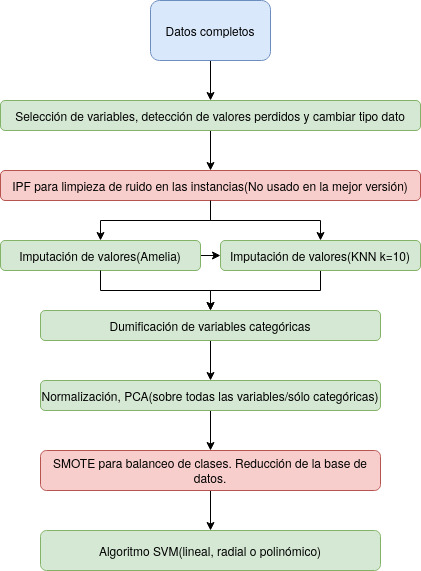
\includegraphics[width=0.5\linewidth]{figures/DiagramaFlujoSVM}
	\caption{Verde: Utilizado en el mejor modelo}
	\label{fig:diagramaflujosvm}
\end{figure}


\end{frame}


\begin{frame}
\frametitle{Puntuación a lo largo del tiempo de SVM}

\begin{figure}
	\centering
	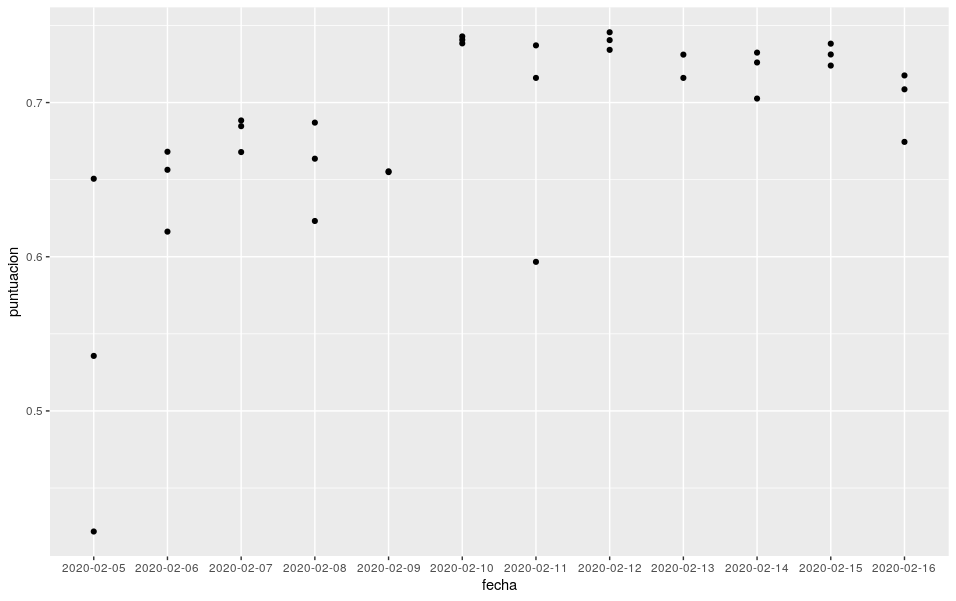
\includegraphics[width=\linewidth]{figures/puntuacionSVM}
	\caption{Máxima puntuación: 74.52\%,  12 de febrero}
	\label{fig:puntuacionsvm}
\end{figure}
Posición final: 2209


\end{frame}